\documentclass[11pt,a4paper]{article}\usepackage[]{graphicx}\usepackage[]{color}
% maxwidth is the original width if it is less than linewidth
% otherwise use linewidth (to make sure the graphics do not exceed the margin)
\makeatletter
\def\maxwidth{ %
  \ifdim\Gin@nat@width>\linewidth
    \linewidth
  \else
    \Gin@nat@width
  \fi
}
\makeatother

\definecolor{fgcolor}{rgb}{0.345, 0.345, 0.345}
\newcommand{\hlnum}[1]{\textcolor[rgb]{0.686,0.059,0.569}{#1}}%
\newcommand{\hlstr}[1]{\textcolor[rgb]{0.192,0.494,0.8}{#1}}%
\newcommand{\hlcom}[1]{\textcolor[rgb]{0.678,0.584,0.686}{\textit{#1}}}%
\newcommand{\hlopt}[1]{\textcolor[rgb]{0,0,0}{#1}}%
\newcommand{\hlstd}[1]{\textcolor[rgb]{0.345,0.345,0.345}{#1}}%
\newcommand{\hlkwa}[1]{\textcolor[rgb]{0.161,0.373,0.58}{\textbf{#1}}}%
\newcommand{\hlkwb}[1]{\textcolor[rgb]{0.69,0.353,0.396}{#1}}%
\newcommand{\hlkwc}[1]{\textcolor[rgb]{0.333,0.667,0.333}{#1}}%
\newcommand{\hlkwd}[1]{\textcolor[rgb]{0.737,0.353,0.396}{\textbf{#1}}}%
\let\hlipl\hlkwb

\usepackage{framed}
\makeatletter
\newenvironment{kframe}{%
 \def\at@end@of@kframe{}%
 \ifinner\ifhmode%
  \def\at@end@of@kframe{\end{minipage}}%
  \begin{minipage}{\columnwidth}%
 \fi\fi%
 \def\FrameCommand##1{\hskip\@totalleftmargin \hskip-\fboxsep
 \colorbox{shadecolor}{##1}\hskip-\fboxsep
     % There is no \\@totalrightmargin, so:
     \hskip-\linewidth \hskip-\@totalleftmargin \hskip\columnwidth}%
 \MakeFramed {\advance\hsize-\width
   \@totalleftmargin\z@ \linewidth\hsize
   \@setminipage}}%
 {\par\unskip\endMakeFramed%
 \at@end@of@kframe}
\makeatother

\definecolor{shadecolor}{rgb}{.97, .97, .97}
\definecolor{messagecolor}{rgb}{0, 0, 0}
\definecolor{warningcolor}{rgb}{1, 0, 1}
\definecolor{errorcolor}{rgb}{1, 0, 0}
\newenvironment{knitrout}{}{} % an empty environment to be redefined in TeX

\usepackage{alltt}
\usepackage[top=1.00in, bottom=1.0in, left=1.1in, right=1.1in]{geometry}
\usepackage{graphicx}
\usepackage[numbers]{natbib}
\bibliographystyle{..//bib/styles/nature.bst}

\usepackage[export]{adjustbox}

%Authors should include answers to the following questions (max. 50 words per question) in a covering letter, to help the Editors decide whether to send the manuscript for peer review:

%What hypotheses or questions does this work address?
%How does this work advance our current understanding of plant science?
%Why is this work important and timely?
%Presubmissions If you are unsure whether your paper falls within the scope of New Phytologist you may submit a presubmission enquiry. Send the abstract of your paper, together with a covering letter that includes answers to the three questions above, to the Managing Editor
\IfFileExists{upquote.sty}{\usepackage{upquote}}{}
\begin{document}


\includegraphics[width=0.5\textwidth, right]{AA_logo.jpg}
\noindent 1300 Centre Street\\
\noindent Boston, MA, 20131\\
% Add a date?


\vspace{1.5ex}



\pagenumbering{gobble}

\noindent{Dear Dr. Pinfield-Wells:}
\vspace{3ex}\\
\noindent Please consider our manuscript entitled `Climate change reshapes the drivers of false spring risk across European trees' as a Full Paper for \textit{New Phytologist}. Climate change has brought renewed interest to late spring freeze events---commonly false springs---which shape the life history of many temperate and boreal plant species. While increased interest has led to a growing number of studies, much of the research takes a simplified view of these events, which has led to contradictory results in how an individual's risk of false spring is changing with warming. By combining multiple, known climatic and geographic factors that contribute to a plant's false spring risk, we assess which predictors most influence risk across species and how these predictors are changing with recent climate change.  \\

\noindent Due to shifts in climate, the onset of biological spring is advancing and tree and shrub species are initiating leafout 4-6 days earlier per $^{\circ}$C of warming \citep{Wolkovich2012, Polgar2014, Fu2015} but last spring freeze dates are not predicted to advance at the same rate as spring onset in some regions \citep{Inouye2008,Martin2010,Labe2016,Wypych2016a,Sgubin2018}. Thus, continued climate change may amplify the effects of false springs, which could affect crucial processes such as carbon uptake and nutrient cycling \citep{Hufkens2012,Richardson2013,Klosterman2018}. By integrating multiple geographic and climatic factors, we may help direct future modelling advancements in false spring research and begin to better understand differences in false spring risk across species. Complex responses to warming and changes in false spring frequency in the future could have escalating impacts on plant community dynamics and further augment climatic shifts. \\

%We find that climate change has fundamentally reshaped the relationships of climatic and geographic factors with false spring risk, while also magnifying species-level variation.  Our results show that a major driver of risk before recent warming---mean spring temperature---has weakened, while the effect of other drivers has reversed.
\noindent \textit{What hypotheses or questions does this work address?} Recent major climate change has increased interest in false spring events, which affect plant performance, survival and shape species distributions. We ask which climatic and geographic factors are the strongest predictors of false springs across six tree species, and how these predictors have shifted with climate change. \\

\noindent \textit{How does this work advance our current understanding of plant science?} By investigating leafout observations of six deciduous tree species from Europe, we unravel the species-specific effects, spring temperature, elevation, distance from the coast and NAO index on false spring risk with climate change. We found that climate-induced warming reshaped the influence of these factors. \\

\noindent \textit{Why is this work important and timely?} Recent studies assess the effects of one predictor (e.g. temperature, elevation or distance from the coast), rendering inconsistent predictions for false springs. Our study shows how robust forecasting must integrate major climatic and geographic factors that underlie false spring, and allow for variation across species and time as warming continues. \\

\noindent Our author team provides an international and interdisciplinary approach to false spring research. The manuscript is 5714 words, with a 200 word summary and four figures. We hope that you will find it suitable for consideration in \textit{New Phytologist}. Thank you for your consideration. \\

\vspace{1.5ex}
\noindent Sincerely, \\
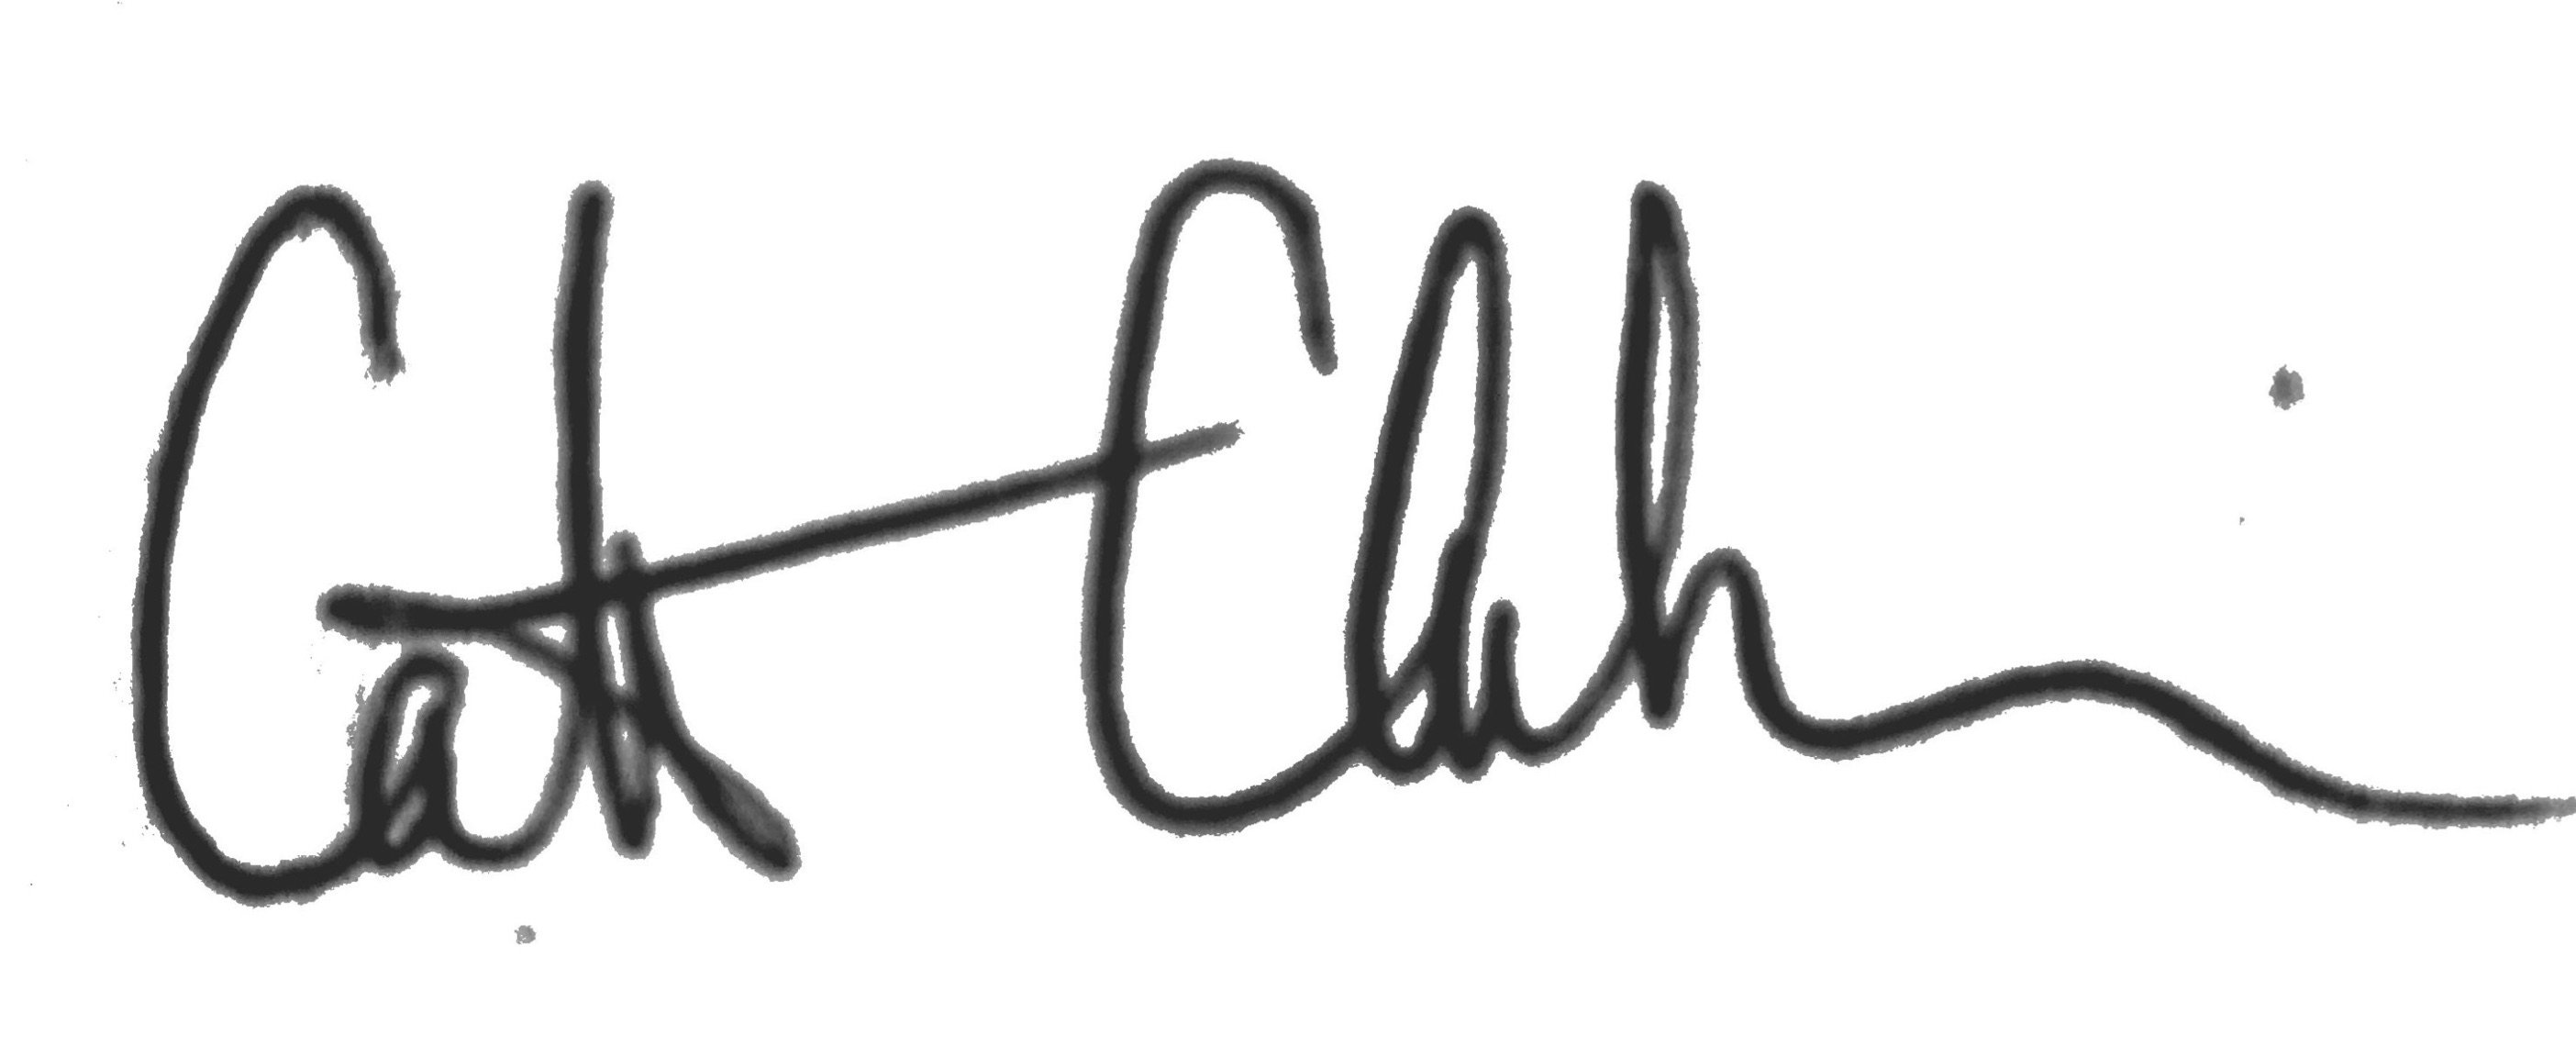
\includegraphics[width=0.2\textwidth]{full_signature.jpg} \\
\noindent Catherine Chamberlain (on behalf of my co-authors)
\vspace{2ex}\\
\noindent Authors:\\
C. J. Chamberlain $^{1,2}$, B. I. Cook $^{3}$, I. Morales-Castilla $^{4,5}$ \& E. M. Wolkovich $^{1,2,6}$
\vspace{2ex}\\
\emph{Author affiliations:}\\
$^{1}$Arnold Arboretum of Harvard University, 1300 Centre Street, Boston, Massachusetts, USA; \\
$^{2}$Organismic \& Evolutionary Biology, Harvard University, 26 Oxford Street, Cambridge, Massachusetts, USA; \\
$^{3}$NASA Goddard Institute for Space Studies, New York, New York, USA; \\
$^{4}$GloCEE - Global Change Ecology and Evolution Group, Department of Life Sciences, Universidad de Alcal\'{a}, Alcal\'{a} de Henares, 28805, Spain \\
$^{5}$Department of Environmental Science and Policy, George Mason University, Fairfax, VA 22030; \\
$^{6}$Forest \& Conservation Sciences, Faculty of Forestry, University of British Columbia, 2424 Main Mall, Vancouver, BC V6T 1Z4\\
\vspace{2ex}
$^*$Corresponding author: 248.953.0189; cchamberlain@g.harvard.edu\\

\bibliography{..//bib/regionalrisk.bib}

\end{document}
